

%%% This LaTeX source document can be used as the basis for your technical
%%% report. Intentionally stripped and simplified
%%% and commands should be adjusted for your particular paper - title, 
%%% author, citations, equations, etc.
% % Citations/references are in report.bib 

\documentclass[conference,backref=page]{acmsiggraph}

\TOGonlineid{45678}
\TOGvolume{0}
\TOGnumber{0}
\TOGarticleDOI{1111111.2222222}
\TOGprojectURL{}
\TOGvideoURL{}
\TOGdataURL{}
\TOGcodeURL{}

% Include this so that citations show up in blue and the page information is included in the reference section
\hypersetup{
    colorlinks = true, 
    linkcolor = blue,
    anchorcolor = red,
    citecolor = blue, 
    filecolor = red, 
}


\title{Milestone 2 Report}

\author{Neil Notman \thanks{e-mail:40124066@live.napier.ac.uk} \\
Edinburgh Napier University\\
Advanced Games Engineering(SET10110) \\
\url{http://nn1098.github.io/adved-games/github-pages/}}
\pdfauthor{Neil Notman}

\keywords{Game, Engine, racing, space}

\begin{document}

\teaser{
   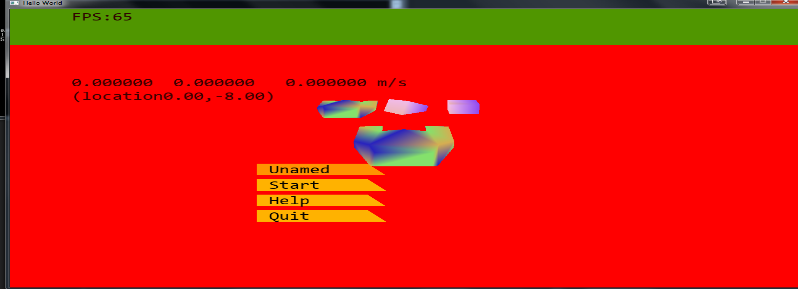
\includegraphics[height=1.5in]{images/mainmenu}
   \caption{This is the main menu screen of the game}
   \label{fig:mainmenu}
 }

\maketitle


\keywordlist

%% Use this only if you're preparing a technical paper to be published in the 
%% ACM 'Transactions on Graphics' journal.

% \TOGlinkslist

% \copyrightspace


\section{Introduction}
The aim of this report and following implementation is to create a game with that conforms to industry standards and contains an agreed list of key functions the report will be used to detail current features and list future work for the next milestone.

This project was initially based as a group however this has now been reduced to a solo implementation which has strained the developement process due to the splitting of work and use of engine developed by the group however the focus for the remainder of the project will be on key features for playability of the game.     

The game itself is currently unnamed but the original idea was for the game to be a 3d space based racer with area's for both racing and free flight with multi-player functionality this will feature a split screen mode.   

\section{Current features}
The game currently features a full menu system including the help menu and ability to render the current controls which is shown below:

\begin{figure}[ht!]
  \includegraphics[height=1.3in]{images/helpmenu}
  \caption{This shows the help menu and controls}
  \label{fig:helpmenu}
\end{figure}

There is graphical developments such as model loading mesh and font rendering with a variety of basic shaders to allow this will be developed further towards the final release to improve the look of the game.  
\nolinebreak
\\\\There are multiple input methods including command parsing using the command line there is also gamepad input and keyboard handling which allows for movement of the player with velocity based integration.
\nolinebreak
\\\\There is basic sound loading and playing functionality provided by the FMOD API. 
\nolinebreak
\\\\The red plane shown in \ref{fig:mainmenu} is redrawn based on the current position of the player this gives the effect of a horizon and will be utilised to spearate the racing and flying elements of the game.

\section{features for milestone 3}
As work continues towards the next milestone the main focus will be getting the racing and flying elements implemented with start and end point to give the game an end state and AI to give the player competition also as shown in \ref{fig:planning} there are some features which have been selected to be excluded from the game as these are non key components as they add to the game rather than add gameplay elements. 

\begin{figure}[ht!]
	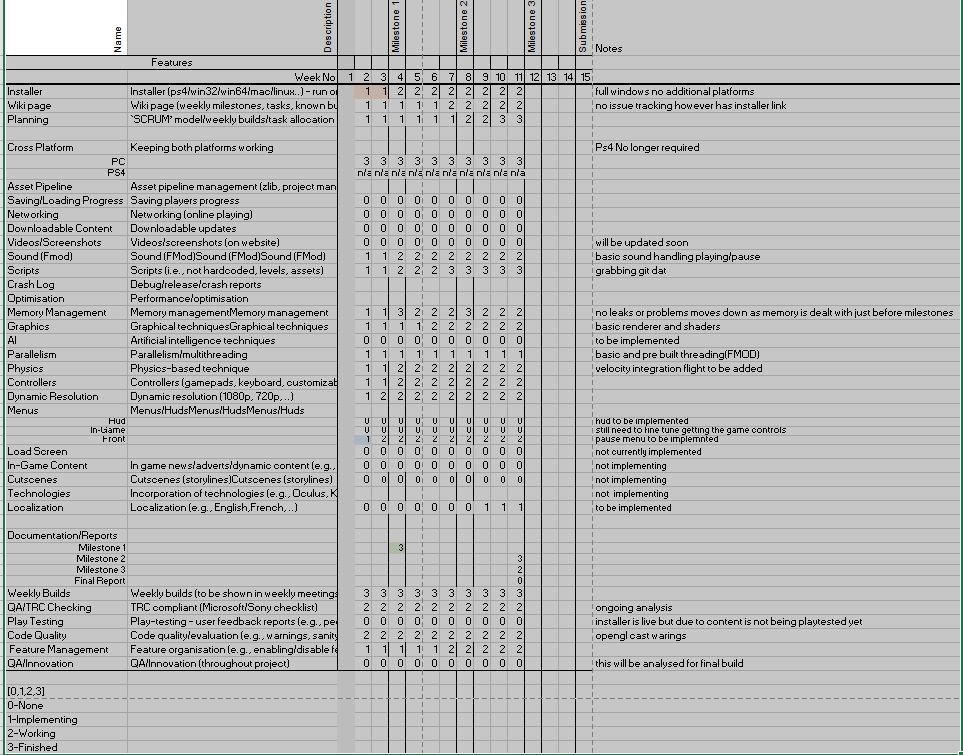
\includegraphics[height=6.0in]{images/planning}
	\caption{This is full feature list and weekly progress}
	\label{fig:planning}
\end{figure}

\end{document}

